%!TEX root = stoh_modeling.tex
\section{Модель}

В данной работе будут рассмотрены 5 основных видов реакций в процессе экспрессии генов:
\begin{itemize}
  \item Присоединение и отсоединение транскрипционных факторов (Рис. \ref{fig:geene_exp1})
  \item Начало транскрипции (Рис. \ref{fig:geene_exp2})
  \item Трансляция (Рис. \ref{fig:geene_exp2})
  \item Деградация белка и тф (Рис. \ref{fig:geene_exp3})
  \item Диффузия между ядрами (Рис. \ref{fig:geene_exp3})
\end{itemize}


\begin{figure}[!h]
  \center{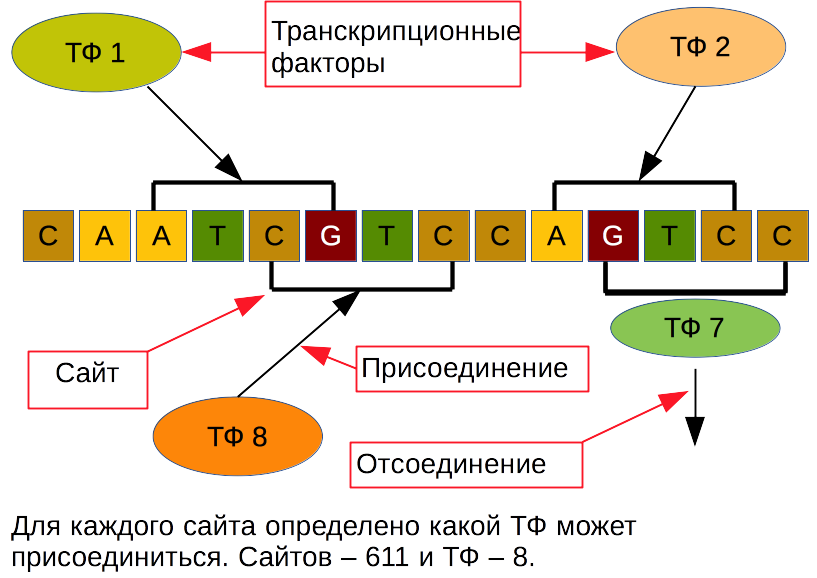
\includegraphics[width=1\linewidth]{geene_exp1}}
  \caption{Процесс присоединения и отсоединения ТФ}
  \label{fig:geene_exp1}
\end{figure}

\begin{figure}[!h]
  \center{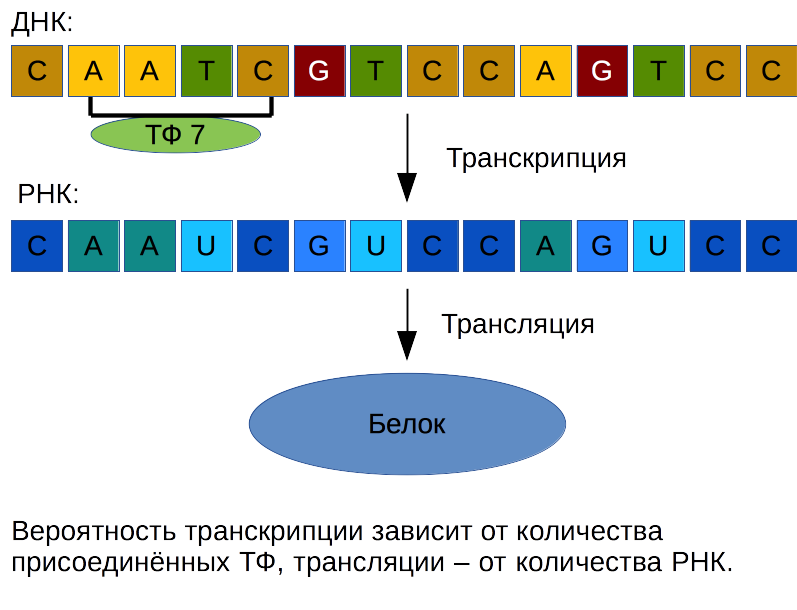
\includegraphics[width=1\linewidth]{geene_exp2}}
  \caption{Процесс транскрипции и трансляции}
  \label{fig:geene_exp2}
\end{figure}

\begin{figure}[!h]
  \center{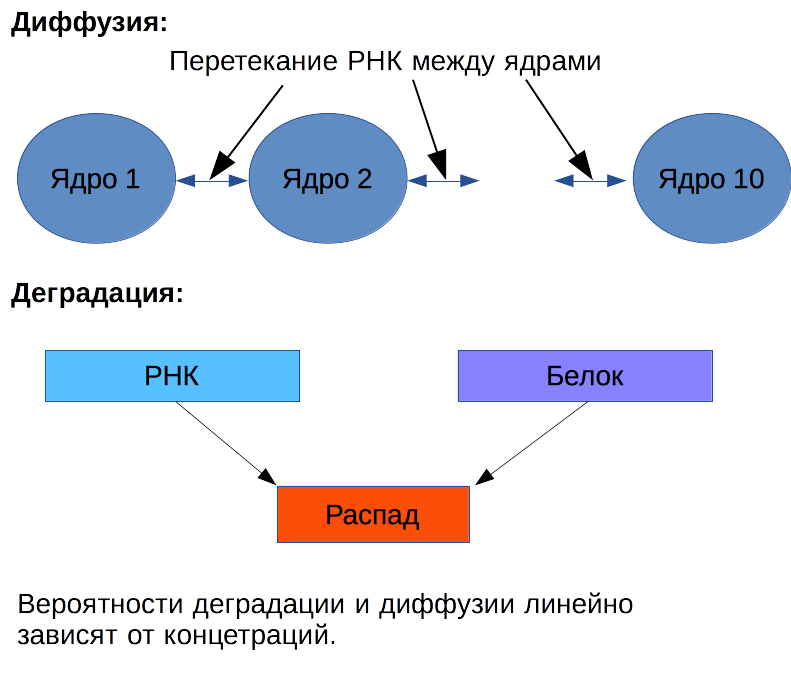
\includegraphics[width=1\linewidth]{geene_exp3}}
  \caption{Процесс диффузии и деградации}
  \label{fig:geene_exp3}
\end{figure}
